\section{Software project management}
\subsection{What is Software Project Management}
Software project management ist essenziell um
\begin{itemize}
	\item Software pünktlich zu liefern
	\item Kosten im Budget zu halten
	\item Software zu liefern, die die Erwartungen der Kunden erfüllen
	\item ein gut funktionierendes Entwicklungsteam zu erhalten
\end{itemize}
\subsubsection{Important factors}
\begin{itemize}
	\item Firmengröße
	\item Software-Kunden
	\item Softwaregröße
	\item Organisationskultur
	\item Software development processes
\end{itemize}
\subsubsection{Main activities}
\begin{itemize}
	\item Projektplanung
	\item Risikomanagement
	\item People-Management
	\item Meldung
	\item Vorschlägeschreiben
\end{itemize}
\subsubsection{Project management triangle}
\begin{table}[H]
\caption{Project management triangle}
\begin{center}
	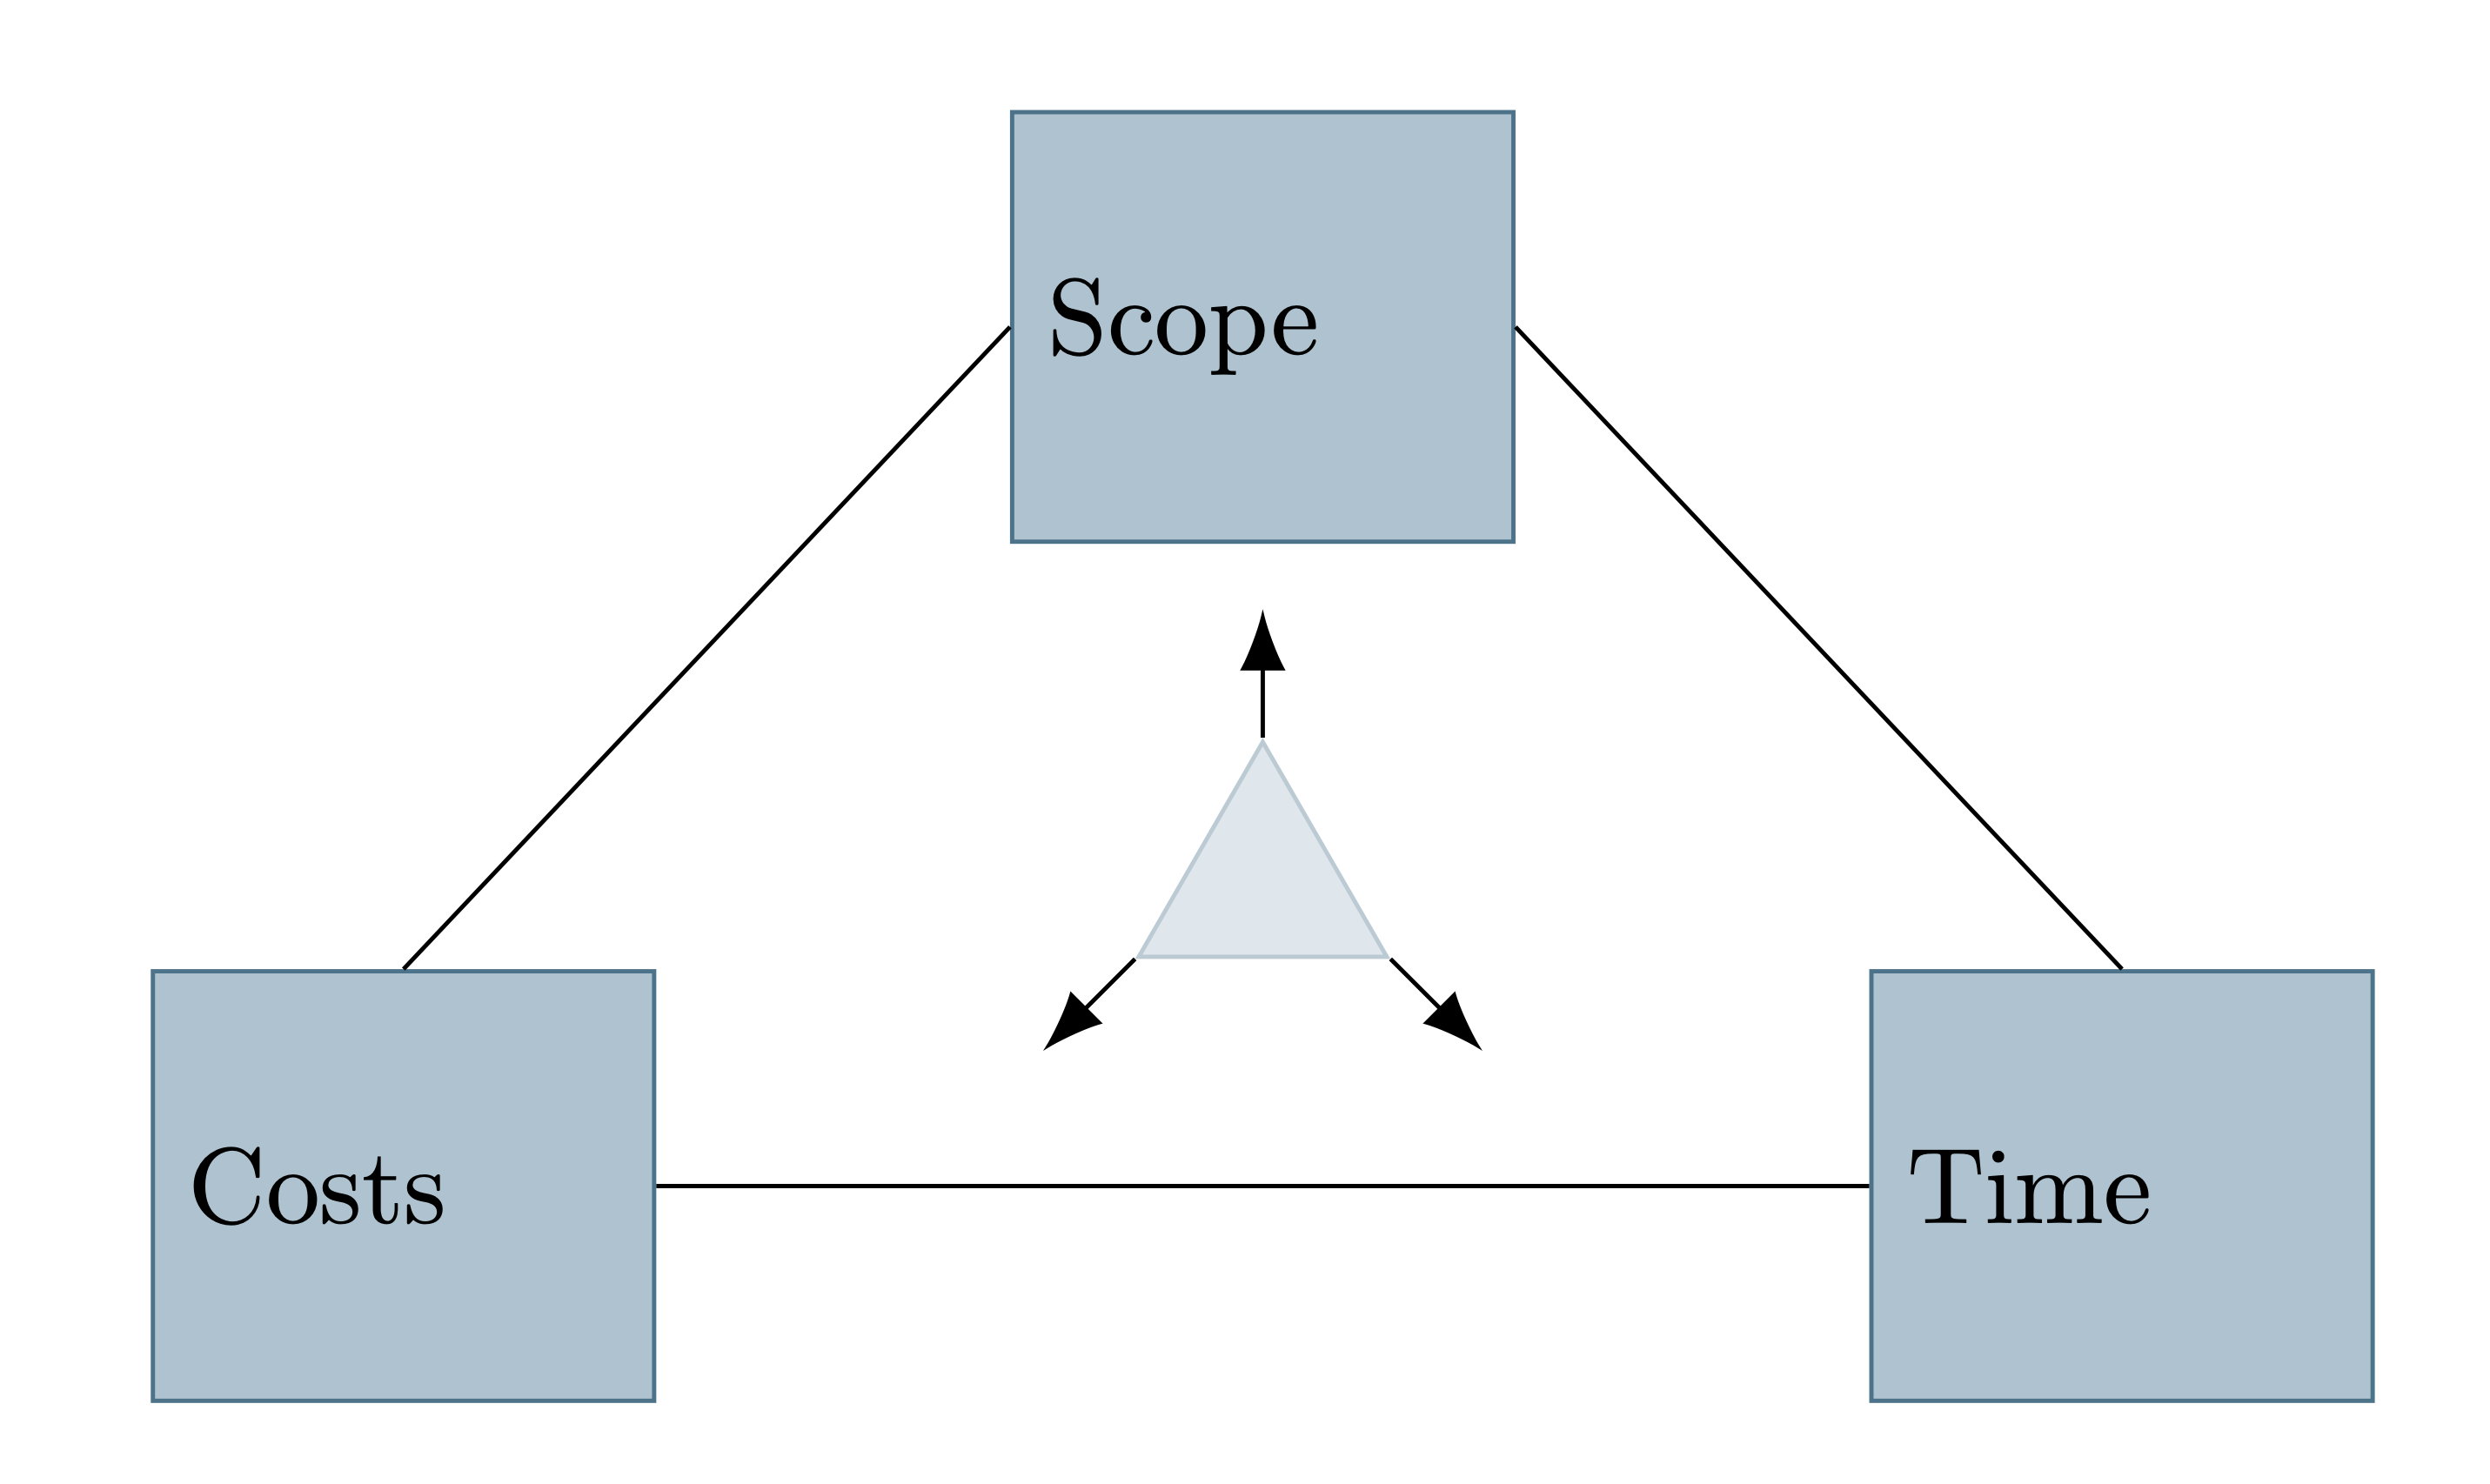
\includegraphics[scale=0.25]{Project_,management_triangle.png}
\end{center}	
\end{table}
Änderung einer Einschränkung verändert die Werte der anderen 
\subsubsection{Five smart criteria}
\begin{itemize}
	\item Spezifisch
	\item Messbar 
	\item Assignable 
	\item Realistisch
	\item Zeitabhängig
\end{itemize}
\subsection{Time management}
\subsubsection{Project scheduling}
\begin{itemize}
	\item Wie wird die Arbeit in separate Aufgaben aufgeteilt
	\item Wann und wie werden diese Aufgaben bearbeitet
	\item Wer die Aufgaben zugeschrieben bekommt
	\item Wie viel Zeit ist nötig um eine Aufgabe zu erledigen
	\item Welche Hardware- und Softwareresourcen werden benötigt
\end{itemize}
\subsubsection{Activity-on-arrow diagram}
\begin{table}[H]
\caption{AoA diagram}
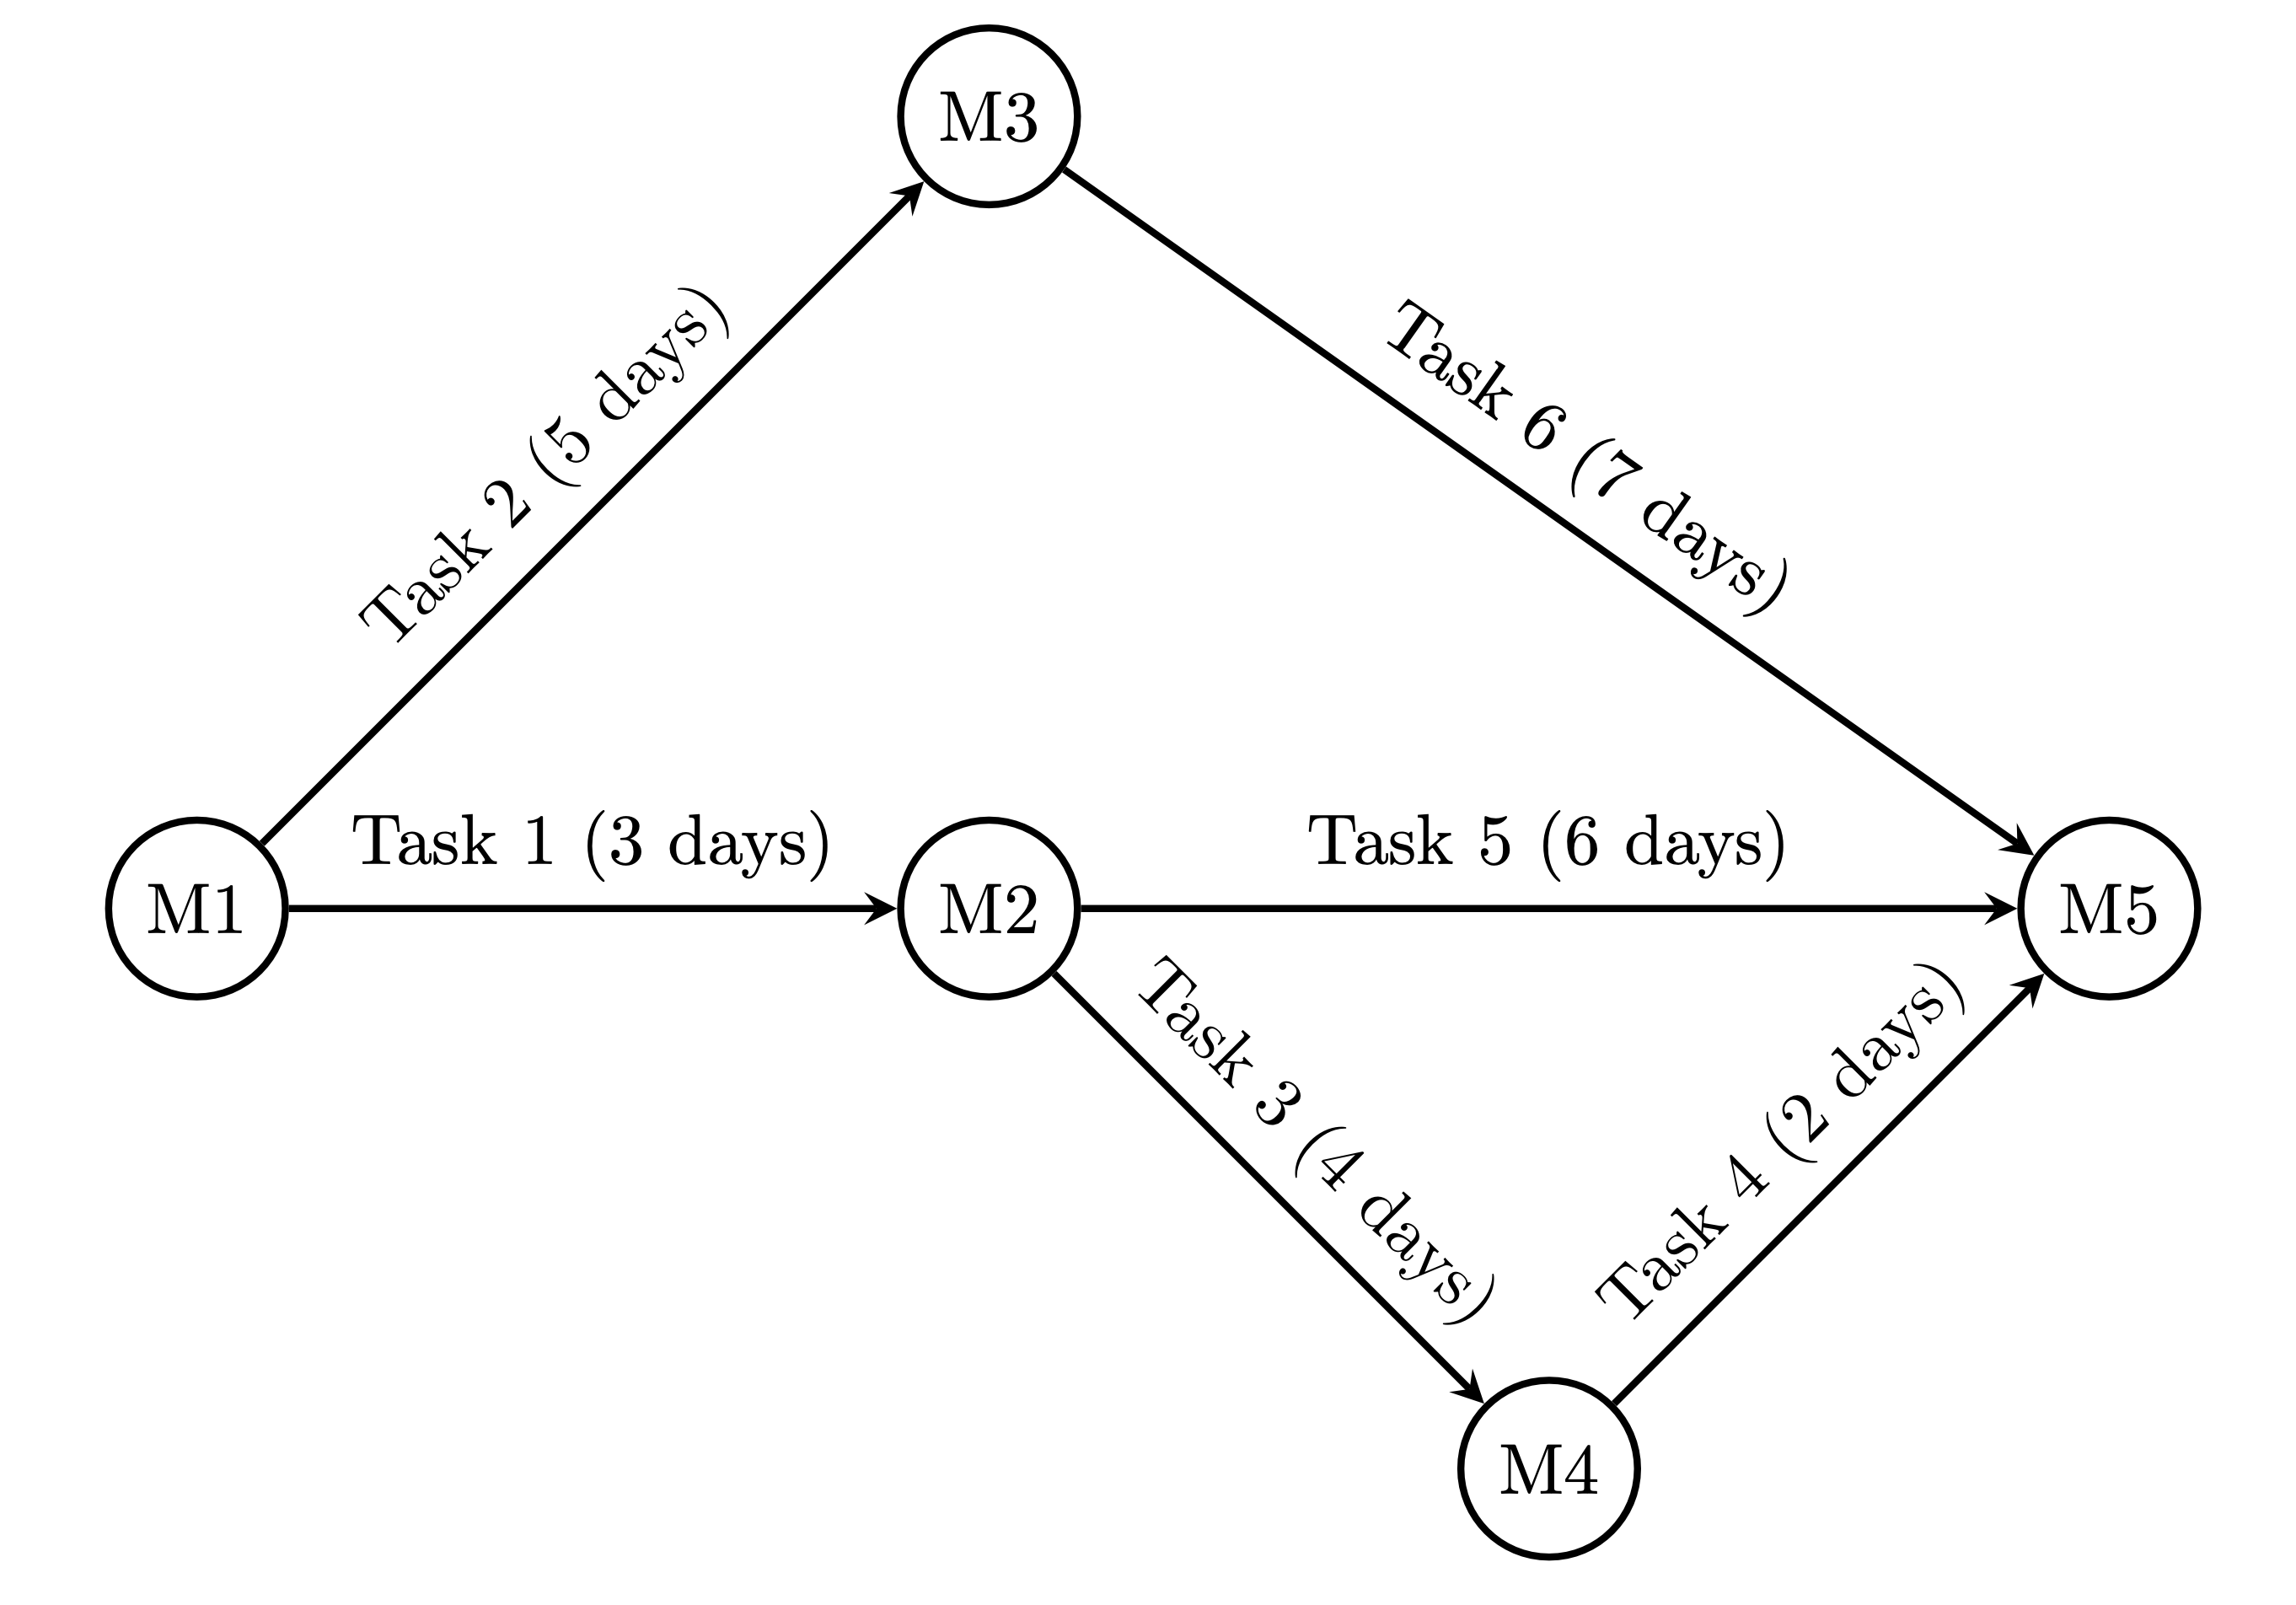
\includegraphics[scale=0.25]{AOA_diagram.png}
\end{table}
\begin{itemize}
	\item Knoten: Milestones
	\item Pfeile: Aktivitäten
\end{itemize}
\subsubsection{Activity-on-node diagram}
\begin{table}[H]
\caption{AoN diagram}
\begin{center}
	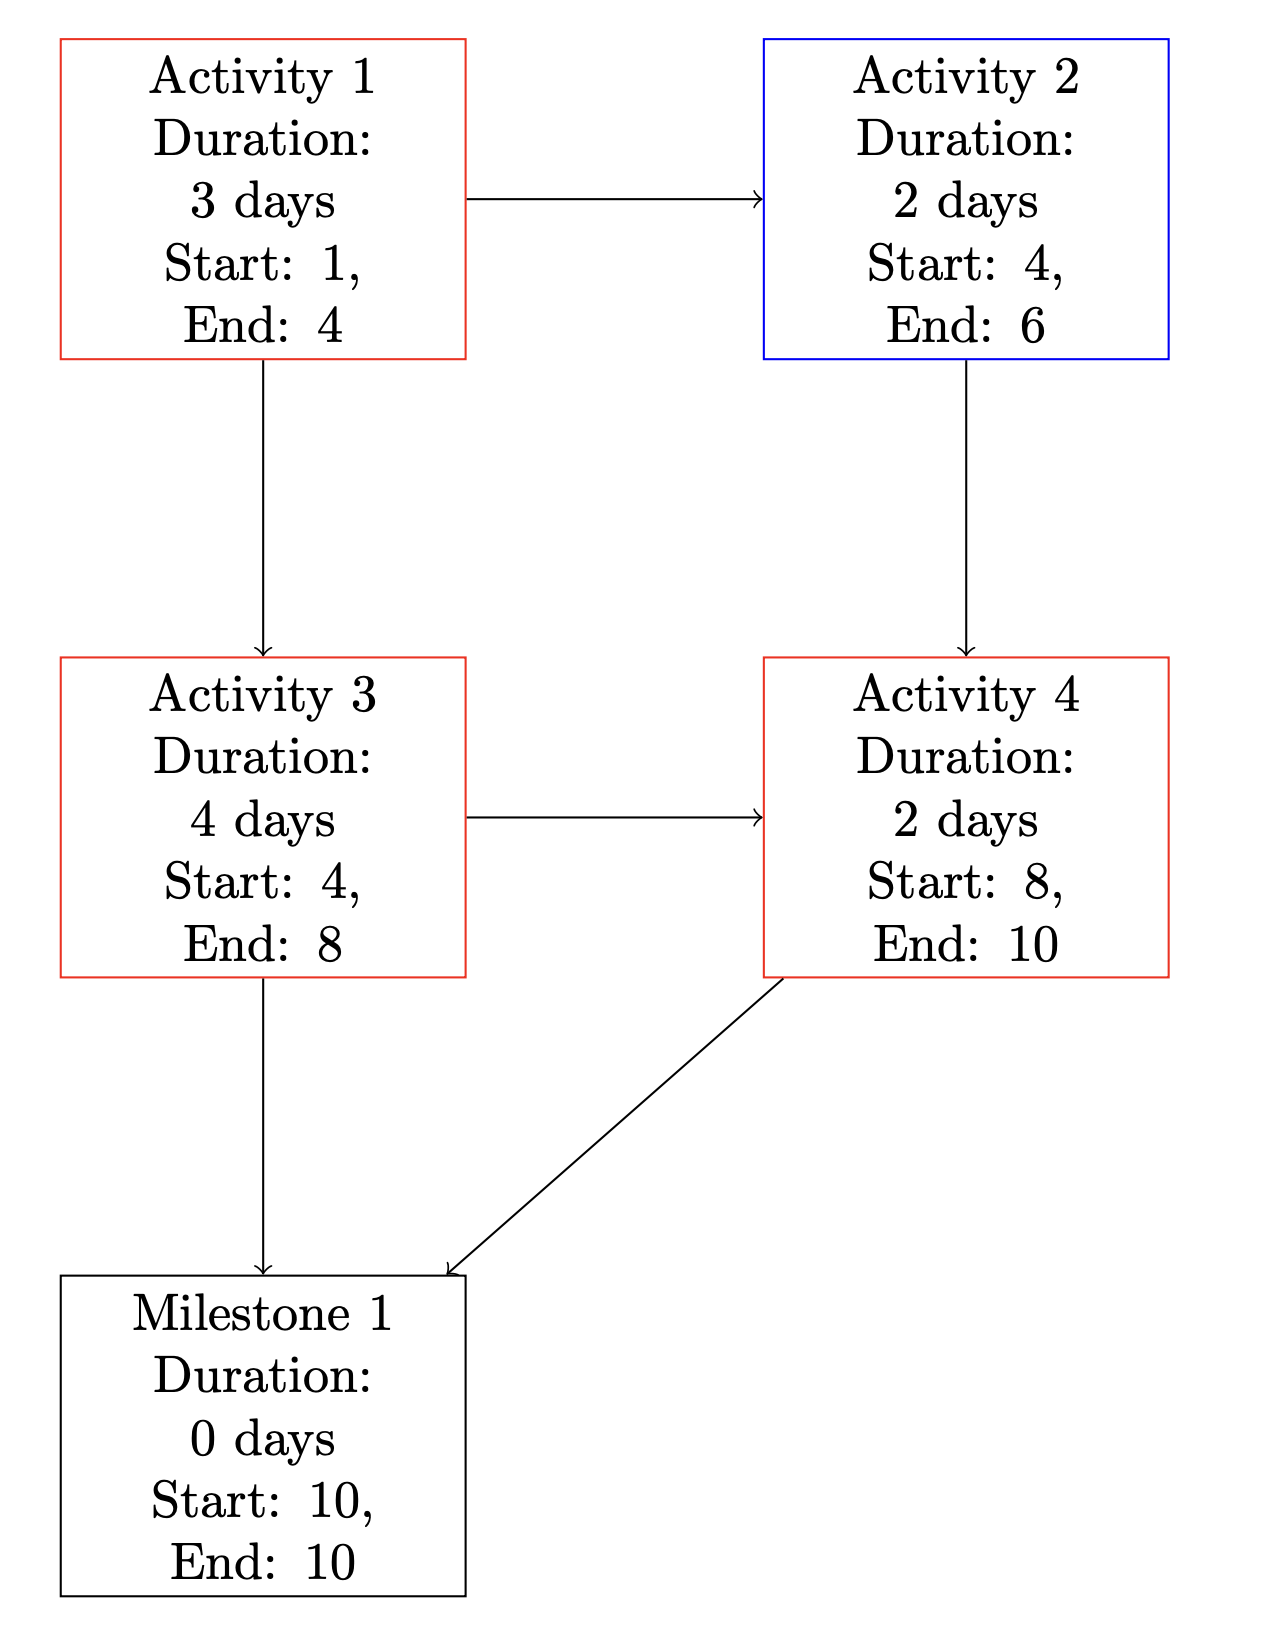
\includegraphics[scale=0.25]{AON_diagram.png}
	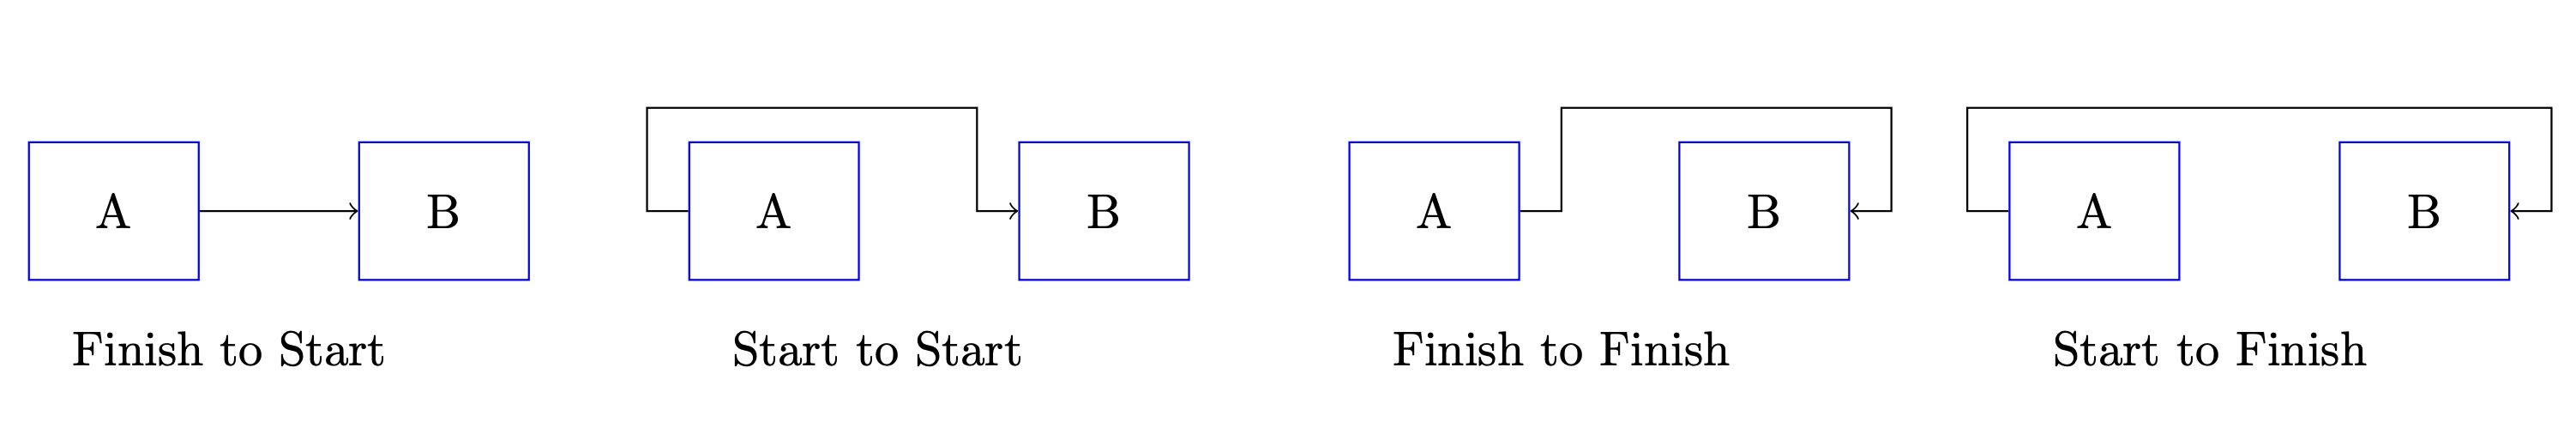
\includegraphics[scale=0.25]{AON_relations.png}
\end{center}
\end{table}
\begin{itemize}
	\item F $\to$ S: B kann erst beginnen, wenn A fertig ist
	\item S $\to$ S: B kann erst beginnen, wenn A begonnen hat
	\item F $\to$ F: B kann erst enden, wenn A beendet ist
	\item S $\to$ F: B kann erst enden, wenn A begonnen hat
\end{itemize}
Die benötigte Zeit für einen Durchlauf kann anhand des kritischen Pfades + die Zeit für alle Aufgaben berechnet werden 
\subsubsection{Gnatt chart}
\begin{table}[H]
\caption{Gantt chart}
\begin{center}
	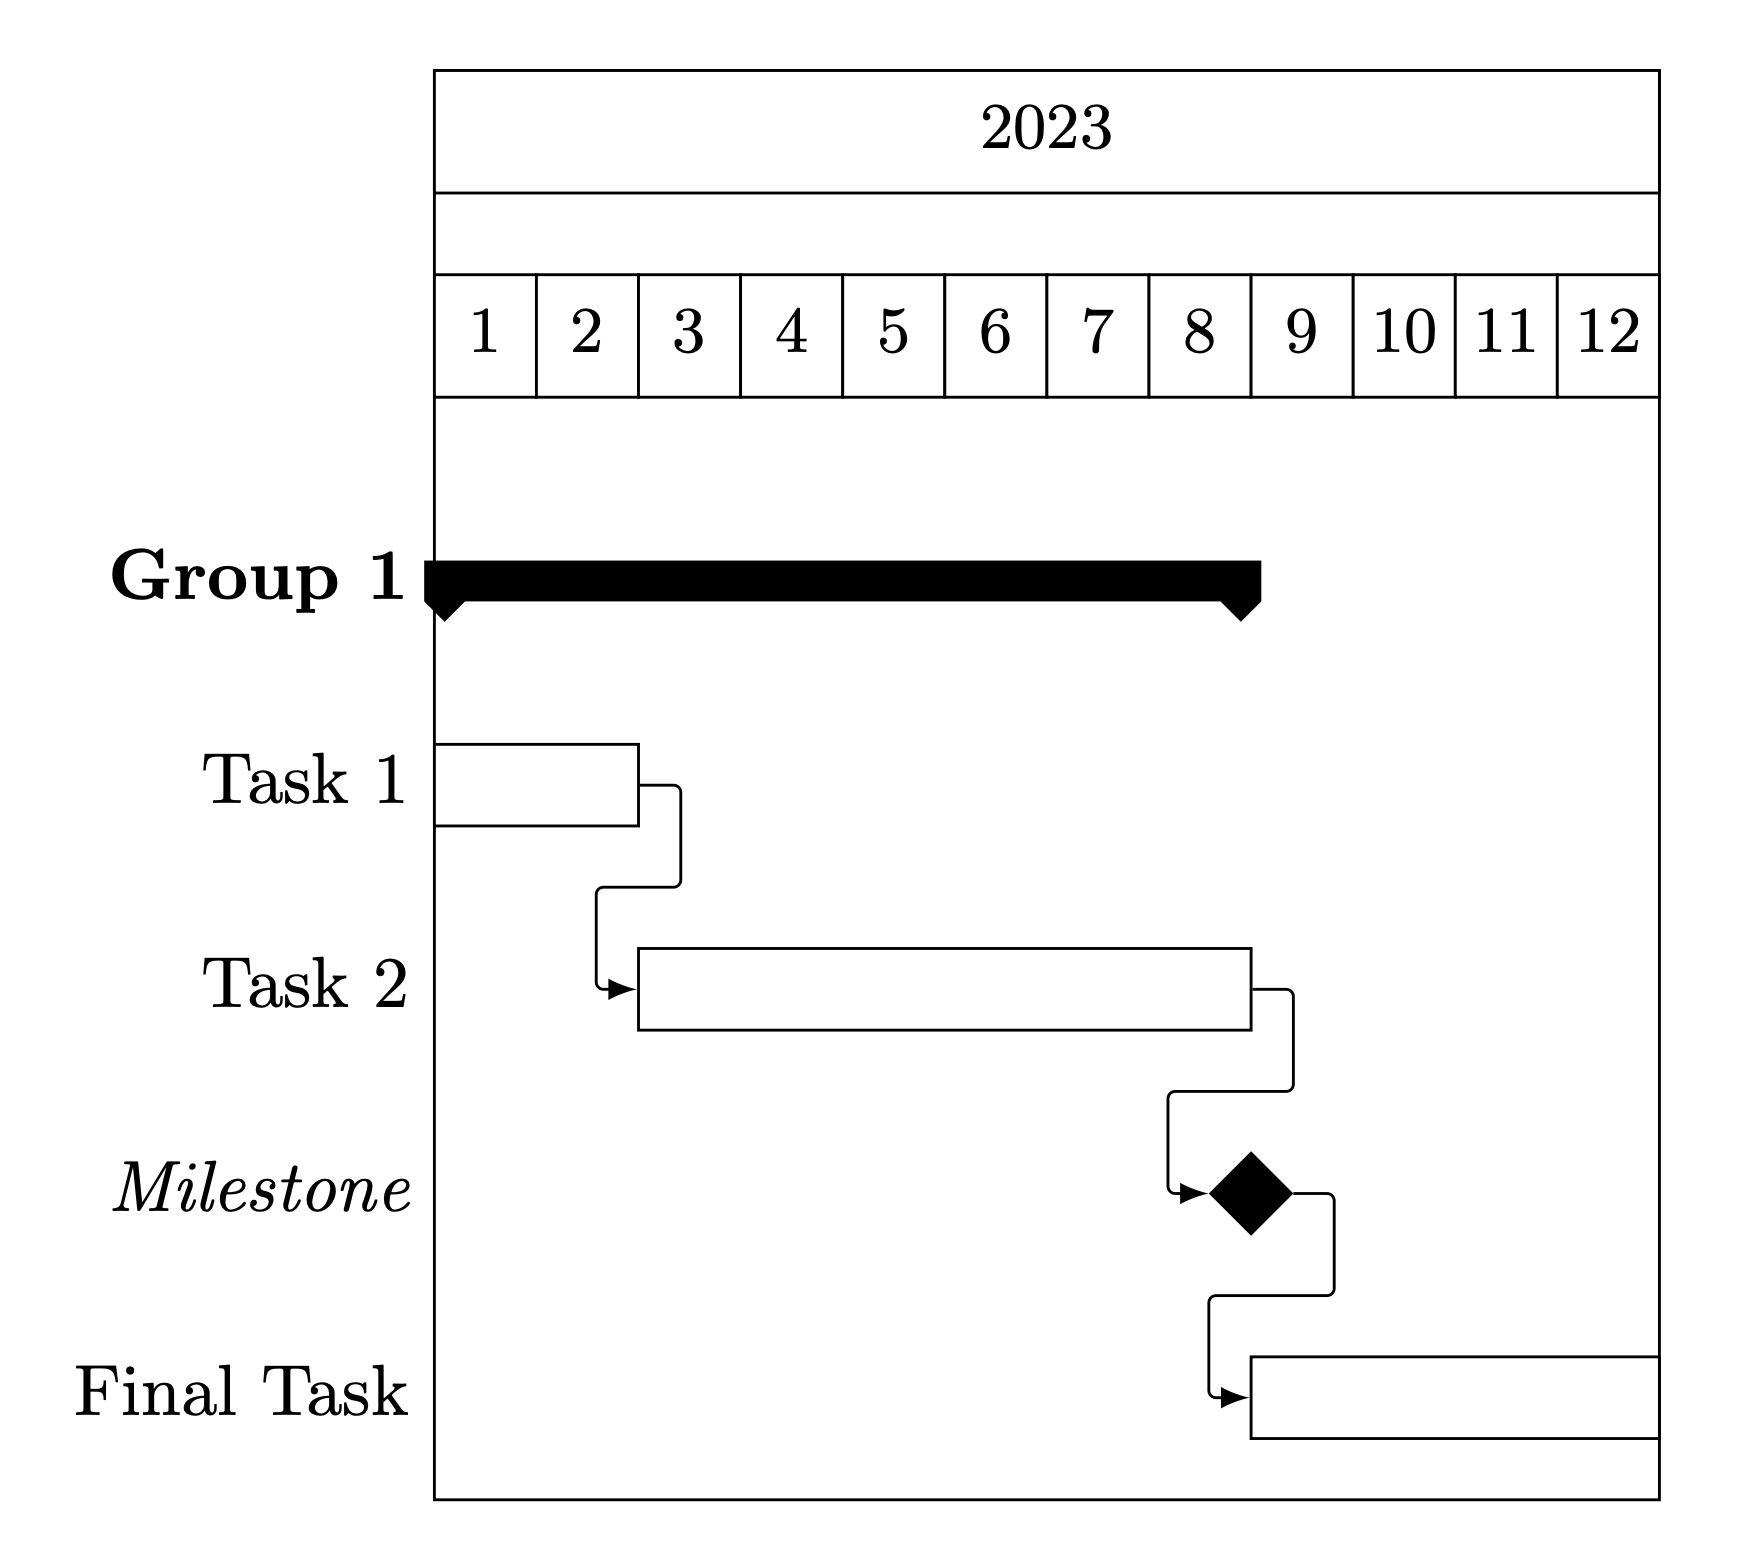
\includegraphics[scale=0.25]{Gnatt.png}
\end{center}	
\end{table}
\subsection{Cost Management}
\subsubsection{Activities}
\begin{itemize}
	\item Kostenmanagement planen
	\item Kosten schätzen
	\item Budget festlegen
	\item Kosten kontrollieren
\end{itemize}
\subsubsection{Algorithmic cost modeling}
$$
	\text{Effort} = A \cdot \text{Size}^B \cdot M
$$
\begin{itemize}
	\item A: Konstante (Orga-Praktiken)
	\item Size: Normally number of lines
	\item B: Complexity
	\item M: Konstante (Erfahrung des Teams)
\end{itemize}
\subsubsection{COCOMO II}
\begin{itemize}
	\item Application composition model: Application points
		$$
			PM = (NAP\cdot(1-\%reuse/100))/PROD
		$$
		\begin{itemize}
			\item PM: Aufwand in person-months
			\item NAP: Anzahl an application points
			\item \%reuse: Wiederverwendeter Code
			\item PROD: NAP/month
		\end{itemize}
	\item Early design model: Function points
		$$
			\text{Effort} = A \cdot \text{Size}^B \cdot M
		$$
	\item Reuse model: Lines of code
		$$
			\text{Effort} = A \cdot \text{Size}^B \cdot M
		$$
	\item Post-architecture model: Lines of code
		$$
			\text{Effort} = A \cdot \text{Size}^B \cdot M
		$$
\end{itemize}
\subsubsection{Improvements}
\begin{itemize}
	\item Data driven
	\item Sensitive analysis
	\item Multiple techniques
	\item Groupe estimates
	\item Training and reflection
	\item Estimation and confidence
\end{itemize}
\subsection{Quality Management}
\subsubsection{Product quality characteristics}
\begin{itemize}
	\item Funktionelle Eignung
	\item Performance/Efficiency
	\item Kompatibilität
	\item Verwendbarkeit
	\item Verlässlichkeit
	\item Sicherheit
	\item Erhaltbarkeit
	\item Portability
\end{itemize}
\subsubsection{Software standarts}
Werden während des quality assurance processes ausgewählt oder definiert und sind wichtig, da sie auf Erfahrung basieren, eine Qualitätsbasis definieren und continuity im Prozess sicherstellen. \newline
Es gibt zwei Arten:
\begin{itemize}
	\item Prozessstandarts 
	\item Produktstandarts
\end{itemize}
\subsubsection{Total Quality Management (TQM)}
\begin{itemize}
	\item Moderner Ansatz
	\item Fokussiert sich auf Kundenzufriedenheit
	\item Prozessverbesserungen durch Problemlösen
	\item Maßstäbe festlegen, um objektiv zu urteilen
	\item Entwickeln einer Qualitätskultur 
\end{itemize}
\subsubsection{Software quality control}
\begin{itemize}
	\item Sicherstellen, dass das Endprodukt die funktionalen und nicht-funktionalen Anforderungen erfüllt
	\item Verwendet software inspections $\to$ software tests
	\item Nutzt Prevention, wie casual analysis meetings
\end{itemize}
\subsubsection{Software Quality Assurance}
\begin{itemize}
	\item Quality assurance group ist vom Entwicklungsteam unabhängig
	\item Bietet unabhängige Meinungen zur Qualität des Produkts
	\item Stimme der Verbraucher
	\item Stellt sicher, dass Qualität in jedem Schritt berücksichtigt wird
	\item Bietet dem Management Transparenz im Prozess und dem Produkt
	\item Conducts audits
\end{itemize}
\subsection{Human Resource Management}
\subsubsection{Managing people}
\begin{itemize}
	\item Rekrutieren und behalten guter Angestellter ist teuer
	\item Stellt sicher, das Entwickler produktiv sind
	\item Teams motivieren und anführen 🤣
\end{itemize}
\subsubsection{Motivating people}
\begin{table}[H]
\caption{Motivation pyramid}
\begin{center}
	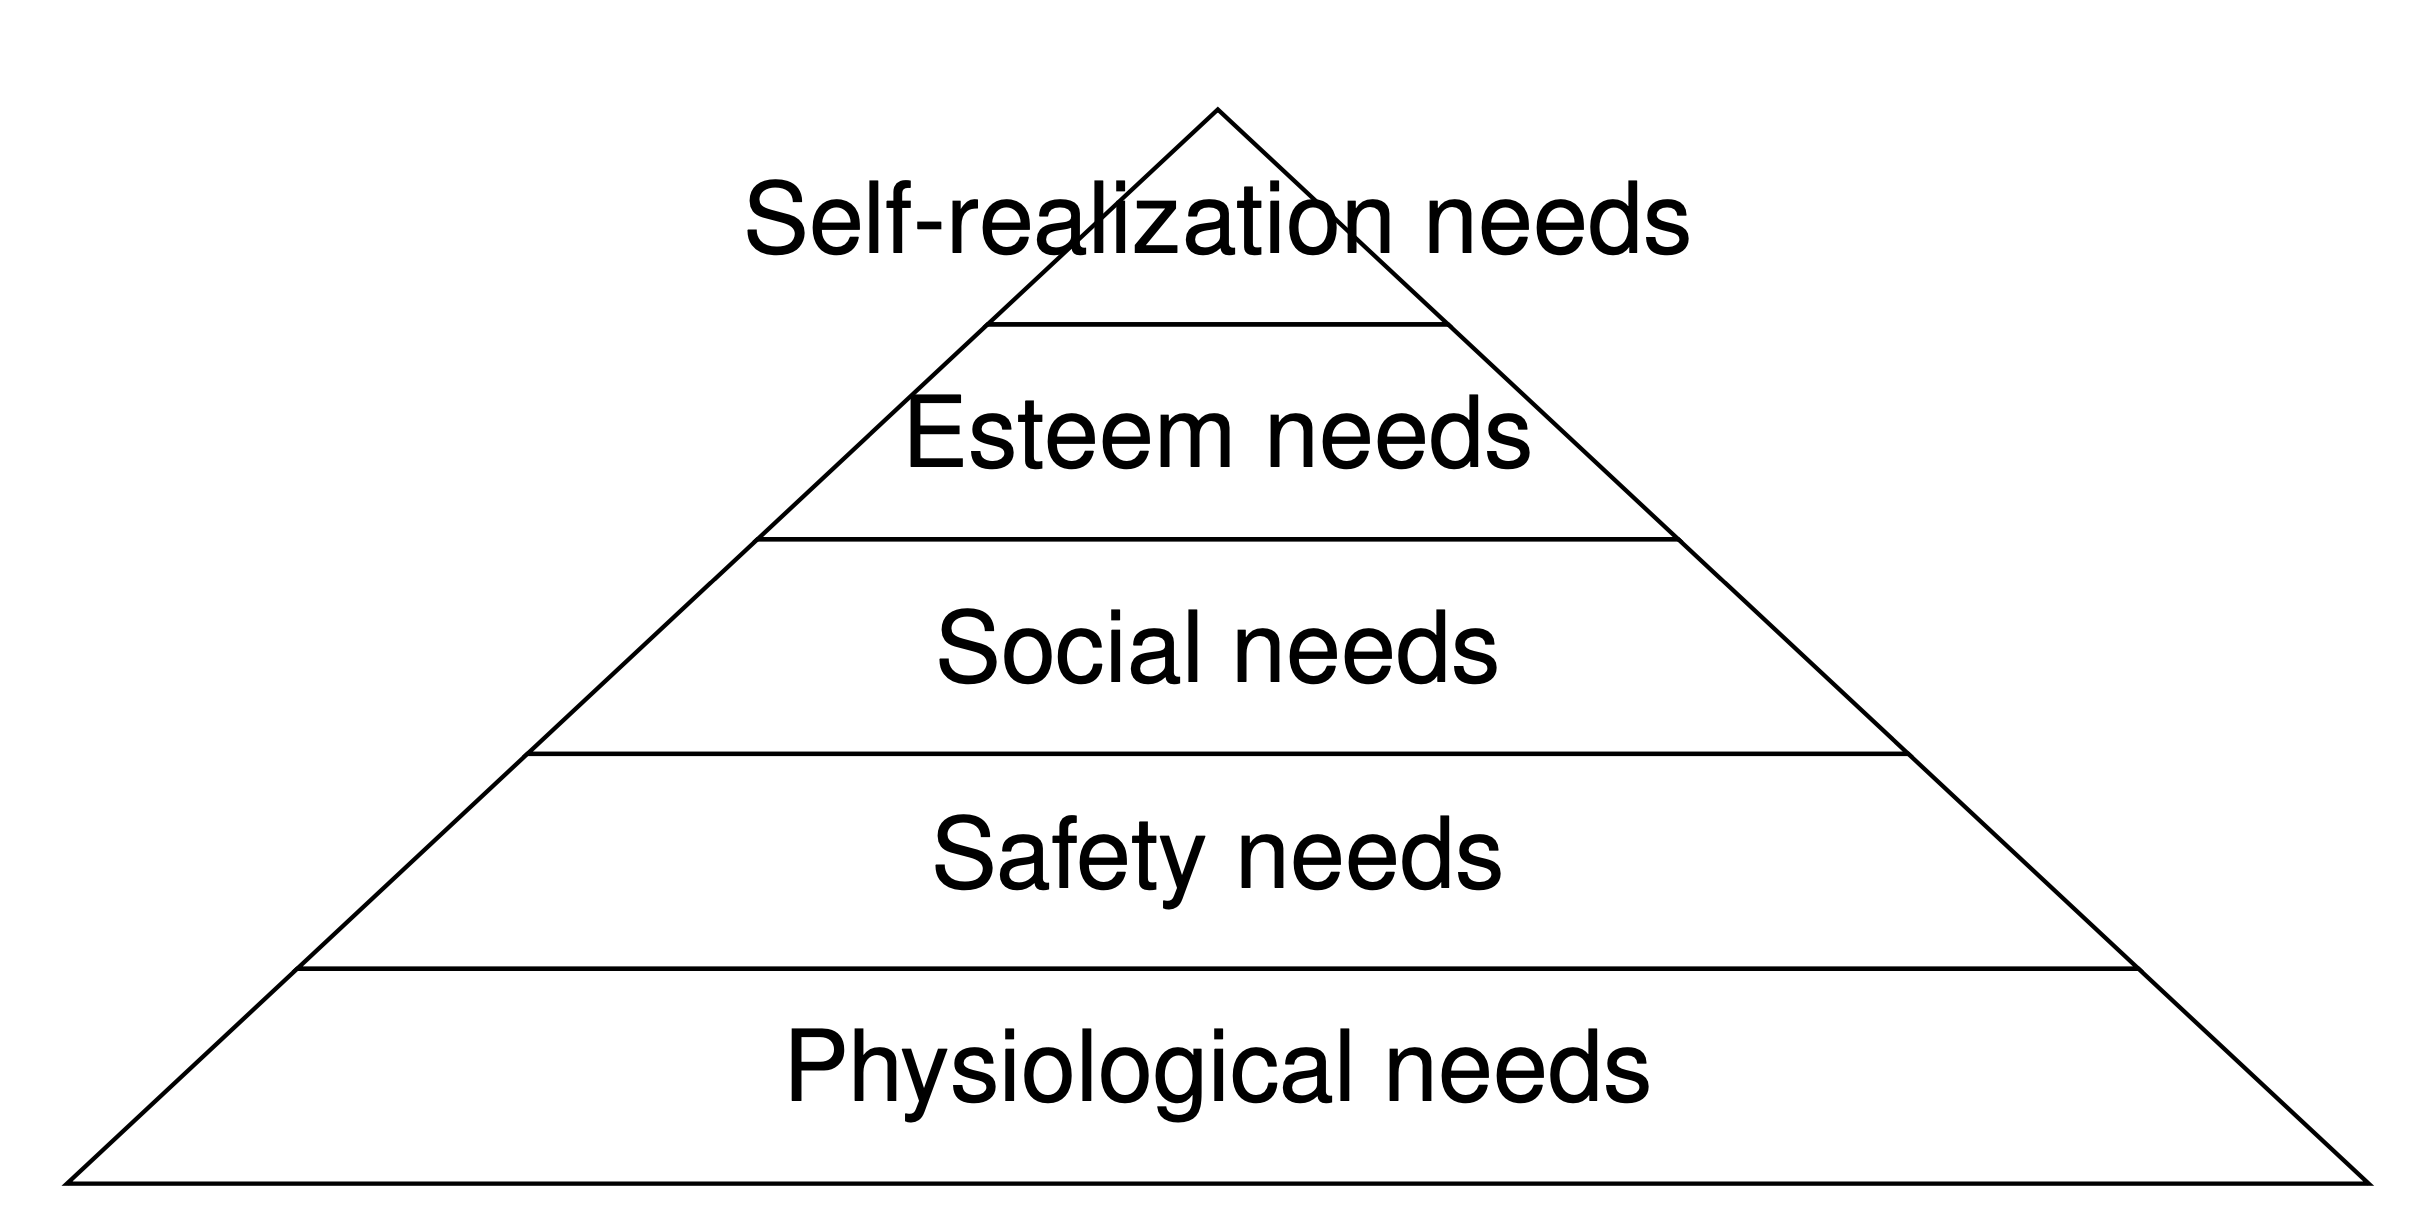
\includegraphics[scale=0.25]{Motivation_pyramid.png}
\end{center}	
\end{table}
Es gibt drei Arten von Menschen:
\begin{itemize}
	\item Aufgabenorientiert: Intellektuelle Challenge 
	\item Selbstorientiert: Persönlicher Erfolg
	\item Interaktionsorientiert: Aktionen Anderer
\end{itemize}
\subsubsection{Teamwork}
Gruppen sollten aus 4-6, max 12 Personen bestehen \newline
$\bold{Cohensive}$ $\bold{groupe}$:
\begin{itemize}
	\item Die Gruppe ist wichtiger als das Individuum
	\item Mitglieder identifizieren sich mit anderen Mitgliedern oder Zielen
	\item Mitglieder stellen Gruppe als Einheit dar
\end{itemize}
Um eine gute Teamchemie zu erzeugen sollten alle Persönlichkeitstypen ausgeglichen in einem Team vertreten sein. Man muss sicherstellen, dass sich die Entwickler nicht als Konkurrenz wahrnehmen
\subsubsection{Group organization}
\begin{itemize}
	\item Informal group
		\begin{itemize}
			\item Ein erfahrener Entwickler im Team kann dieses sehr effektiv machen
			\item Neue unerfahrener Mitglieder können Koordination stören
		\end{itemize}
	\item Hierarchical group
		\begin{itemize}
			\item Können bei gut verstanden Problemen sehr schnell arbeiten
			\item Schlecht bei komplexen Problemen, da Kommunikation auf jeder Ebene notwendig
		\end{itemize}
\end{itemize} 
\subsection{Risk Management}
\subsubsection{Classes}
\begin{itemize}
	\item Project risk: schedule or resources
	\item Product risk: quality or performance
	\item Business risk: dev. orga. 
\end{itemize}
\subsubsection{Stages of risk management}
\begin{table}[H]
\caption{Risk management}
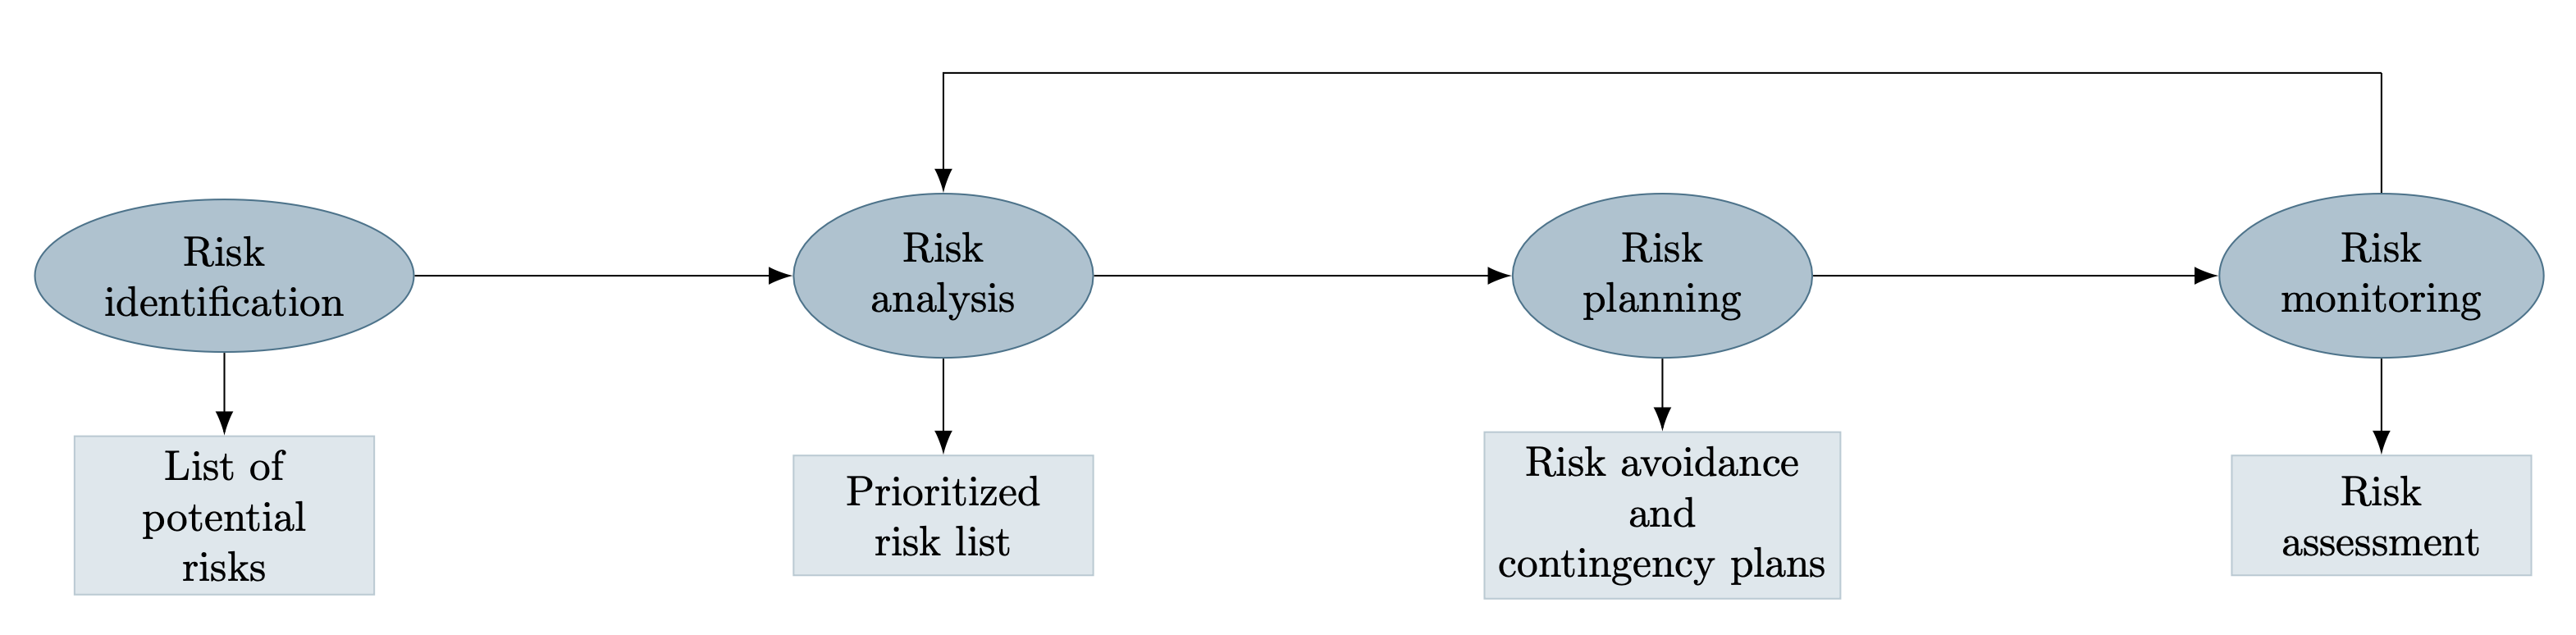
\includegraphics[scale=0.25]{Risk_management.png}	
\end{table}
\subsubsection{Risk management plan}
\begin{itemize}
	\item Ergebnisdokumentation des Risikomanagements
	\item Inklusive Diskussionen und Analysen über die Risiken
	\item Verändert sich während des Projekts
\end{itemize}
\subsubsection{Agile risk management}
\begin{itemize}
	\item Gleiche Grundlage, außer der formalen Dokumentation
	\item Reduziert Anforderungsänderungsrisiken
	\item Anfälliger für project risks, da abhängiger von Menschen  
\end{itemize}
\subsubsection{Risk identification}
\begin{itemize}
	\item Estimation risk
	\item Organizational risk
	\item People risk
	\item Requirements risk
	\item Technology risk
	\item Tool risk
\end{itemize}
Die verschiedenen Risiken müssen hinsichtlich ihrer Wahrscheinlichkeit und Ernsthaftigkeit betrachtet werden
\subsubsection{What if}
\begin{itemize}
	\item Individual risk
	\item Combination of risks
	\item External factors that effect these risks
\end{itemize}
\subsubsection{Risk planning}
\begin{itemize}
	\item Avoidance strategy
	\item Minimization startegies
	\item Contingenzy plans
\end{itemize}



